\chapter{Texture}

\begin{abstract}
    纹理是比直接用颜色值更具有连续性, 对每个光栅化的屏幕坐标(usually a pixel center), 
    算出它的uv坐标(利用三角形顶点重心坐标插值using barycentric coordinates), 
    用uv坐标去查询texture上的颜色值,把这个颜色值当作
    漫反射系数Kd使用albedo Kd(Blinn-Phong reflectance model)
    \begin{enumerate}
        \item \text{for each rasterized screen sample(x,y):}
        \begin{enumerate}
            \item \text{(u,v) = evaluate texture coordinate at (x,y)}
            \item \text{texcolor = texture.sample(u,v)}
            \item \text{set sample's color to texcolor}
        \end{enumerate}
    \end{enumerate}    
\end{abstract}

可阅读
Chapter 20 Textures and Texture Mapping\cite{CGPP3ed}

Chapter 11 Texture Mapping\cite{FCG4ed}

Chapter 6 Texturing\cite{RTR4ed}

\section{Texture Mapping}
纹理映射,即纹理坐标的生成函数,纹理空间之内任意一个二维坐标都在[0,1]之内。

\begin{figure}[h]
    \centering
    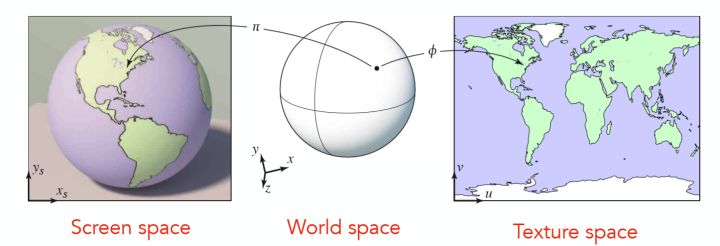
\includegraphics[width=1\textwidth]{images/texture-mapping-sphere.jpg}
    \caption{地球仪}    
\end{figure}

纹理应用在表面的大致逻辑是
\begin{lstlisting}
    Color texture_lookup(Texture t, float u, float v) {
        int i = round(u * t.width() - 0.5);
        int j = round(v * t.height() - 0.5);
        return t.get_pixel(i,j);
    }
    Color shade_surface_point(Surface s, Point p, Texture t) {
        Vector normal = s.get_normal(p);
        (u,v) = s.get_texcoord(p);
        Color diffuse_color = texture_lookup(t, u, v);
        // compute shading using diffuse_color and normal 
        // return shading result    
    }
\end{lstlisting}
就是对每个光栅化的屏幕坐标算出它的uv坐标(利用三角形顶点重心坐标插值),再利用uv坐标取查询texture
上的颜色,把这个颜色信息当作漫反射系数Kd。


以顶视图Y轴方向来看,对X(S)和Z(T)生成对应的纹理坐标值UV,即Y平面为UV展开

\begin{enumerate}
    \item \textsf{遍历所有点得到lowestX和highestX,lowestX=-12.00,highestX=134.56}
    \item \textsf{得到绝对范围 range=(lowest - highest) * -1 = (-12.00-134.56)*-1=146.56}
    \item \textsf{与0的偏移值offset=0-lowestX=0 - (-12.00)=12}
    \item \textsf{vertex x=87.45, absoluteX=X+offset=87.45+12=99.45}
    \item \textsf{get S value, s = absoluteX / range = 99.45/145.56=0.679}
    \item \textsf{do the same for Z axis to get T value}
\end{enumerate}

从Image Space到Texture space(T), 存在一个函数映射,从World space中Surface(S), 数学模型如下:

\begin{align*}
    \phi &: S \rightarrow T \\
    &: (x,y,z) \rightarrow (u,v)
\end{align*}

函数$\phi$存在很多种形式

\subsection{Basic Texturing}

是最基本的纹理映射,仿射粘贴(affine gluing),把图像粘贴到一个三角形,通过三角形的三个顶点指定纹理坐标方式,
顶点存储uv值,并在特定的texture中获取相应的值即可,即最广义的纹理贴图。

\subsection{Planar Projection}


orthographic viewing $M_{t}$是变换矩阵

\begin{align*}
    \phi(x,y,z) = (u,v) \qquad where 
    \begin{bmatrix} u \\ v \\ * \\ 1 \end{bmatrix} = M_{t} 
    \begin{bmatrix} x \\ y \\ z \\ 1 \end{bmatrix}
\end{align*}

perspective viewing $P_{t}$是投影矩阵

\begin{align*}
    \phi(x,y,z) = (u/w,v/w) \qquad where 
    \begin{bmatrix} u \\ v \\ * \\ w \end{bmatrix} = P_{t} 
    \begin{bmatrix} x \\ y \\ z \\ 1 \end{bmatrix}
\end{align*}


\subsection{Sphereical Coordinates}

\begin{equation}
    \phi(x,y,z) = ([\pi+atan2(y,x)]/2\pi,[\pi-acos(z/s\|x\|)]/\pi)
\end{equation}

\subsection{Cylindrical Coordinates}

\begin{align*}
    \phi(x,y,z) = (\frac{1}{2\pi}[\pi+atan2(y,x)]/2\pi,\frac{1}{2}[1+z])
\end{align*}

\subsection{Cubemaps}

纹理可以在围绕被渲染物体的距离上建模环境,如使用6个正方形纹理表示一个环绕场景的大立方体的面,
每个纹理像素表示顺着环境中一个方向看过去的色彩,GLSL提供一个专门的samplerCube数据类型来支持。
在顶点着色过程中,把顶点的材料处理为一个完美镜面并且从合适的入射方向获取环境数据。
\begin{align*}
    \phi(x,y,z) \mapsto (\frac{x}{z},\frac{y}{z})
\end{align*}

\subsection{Interpolated Texture Coordinates }

\begin{description}
    \item [distortion] \textsf{映射关系是一个连续的函数,就存在失真,扭曲,畸变}
    \item [seam] \textsf{拓扑可以展开为平面,但是因为顶点可能有多个uv值,会出现缝隙问题,边界过渡问题}
\end{description}

\subsection{UV Unwrapping}

UV展开就是把物体的表面映射到平面图像上的过程。为了让弯曲的表面信息也能在平面上被精准存放下来,对切割线seam的要求

\section{Normal Mapping}
法线映射,来自一个纹理的rgb数值被当作顶点的法线的xyz,因为法线取值范围是[-1,1],而rgb取值范围是[0,1],法线已纹理
数据存储使会转换
$$
rgb = \frac{normal_xyz}{2.0} + 0.5
$$
在Fragment Shader中需要转换会色彩值
$$
normal_xyz = 2 \times rgb - 1
$$

\section{Texture Sampling}

前面说了纹理映射,如果是一一对应很好理解,找到对应的就行了,但现实中更复杂的是对特别小resolution低,
或特别大resolution高的产生的问题的处理。


\paragraph{low resolution}
纹理小会走样失真,需要一些图像处理技术来处理,
双线性插值Bilinear Interpolation是性价比很高的选择

\paragraph{high resolution}
纹理大会更走样失真,近处是锯齿Jaggies,远处是摩尔纹Moire。从信号的角度来看,就是采样频率过低无法还原信号源。
从透视的近大远小的原因,用远小的像素来表示面片的真实像素,自然会失真。

\paragraph{Upsampling}
上采样,
放大Magnification图像,基本是内插值方法,在原有像素点之间采样某种插值算法插入新的像素

\paragraph{Downsampling}
下(降)采样,
缩小Minification图像,把图像视口变小,原来多个像素的均值作为一个目标像素存储

\paragraph{Supersampling}
超采样,就是一个源像素大到一个区域事,把这个源像素细分为更多的子像素,获取子像素的采样,这种算法的计算量是几何倍数增长

\paragraph{Mipmap}
最理想的方法就是一一对应的查询,Mip comes from the Latin "multum in parvo", meaning a multitude in a small space.


\section{Color Space}
sRGB/RGB color space, linear/gamma space, 

设计师的眼睛与屏幕的显式因素

\section{Bump Map}

Jim Blinn在1978的\text{Simulation of Wrinkled surfaces}论文中使用一种灰度高度图来建模物体表面法线的扰动,扰动法向量的大小用
某些表面参数的偏微分和高度图来计算。要把扰动的法向量加入光照模型中进行计算,就必须是像素级的shading(因为顶点级的Gouraud shading
是逐顶点计算光照公式,最后每个像素都是这些顶点插值出来的,OpenGL的标准光照是基于Phong光照模型但使用Gouraud shading,Phong shading
是指插值顶点法向量在fragment基本计算光照公式)。

Bump Map是Phong Shading的一项扩展,表面法线用来计算顶点的光亮,它必须通过顶点插值来确定,虽然每个fragment都有一个独特的法线,
但法线不能准确表示表面的粗糙程度,而Bump Map就是为了影响法线的改变,最终影响颜色值,所以算是一种负责光方向的纹理映射,
不同的凹凸数据,使用不同的方法来影响法线,常见的有两种模式:
\begin{itemize}
    \item \text{Emboss Bump Map浮雕,使用HeightMap,用在diffuse lighting中}
    \item \text{Environment-mapped,使用grayscale height map}
    \item \text{DOT3 Bumap Map点乘凸凹贴图,使用NormalMap}
\end{itemize}

凹凸贴图通常保存为RGB纹理,纹理每个通道分别存储标准化方向向量的x、y、z轴的值,作为颜色数据,可以像其他的纹理一样,
进行采样插值,不管凹凸贴图分辨率大小,都会存在插值并对每个fragment法线产生作用


\subsection{Height Map}
高度图是存储高度信息的数据,通常计算XY方向上的倾斜度
\begin{gather*}
    x_gradient = pixel(x-1,y) - pixel(x+1,y) \\
    y_gradient = pixel(x,y-1) - pixel(x,y+1) \\
    normalNew = normal + (U * x_gradient) + (V * y_gradient)
\end{gather*}
在的Bump Map\cite{CGPP3ed}中,有一个公式更加通用
\begin{align*}
    n^{'} = S(n + rt_{1} + gt_{2})
\end{align*}
它描述了两个方向上向量对法线的影响

\subsection{EMBM}
环境影射扰动纹理坐标而不是法向量,其输入纹理是一个二维的图像du/dv,其纹理像素表示应用到uv纹理坐标上的偏移量,
就是纹理获取坐标为(u+du,v+dv),其中uv分别表示逐顶点插值的纹理坐标,du/dv是从map中获取的偏移量,这样贷来的限制
是光照必须来自纹理。

\subsection{Normal Map}

实时渲染中目前图像硬件模拟凹凸效果比较通用的方法就是法线贴图,bluish texture偏蓝色纹理,法线贴图在纹理的每个像素中存储一个颜色。
有两种方法生成法线贴图
\paragraph{灰度图}
预先计算每个像素与其垂直和水平相邻像素之间的差别,将两个结果数字(导数)转换为单位法线并存储为颜色
\paragraph{精模烘焙法线}
把纹理的每个像素与精模的表面位置结合起来,将其结果编码为法线存储为颜色值

为使生成的纹理可以在任意旋转下均反复使用,存储的法线必须在\textbf{切线空间}中。为了将切线空间的法线转换到世界空间,需要3个轴形成一个旋转矩阵,面法线N算一个,
\textbf{一个沿着目标多边形的面或与目标多边形曲面相切的切线方向T(为了让切向量与副法线在顶点指向的方向完全一致,使用模型纹理坐标的正X轴方向作为切线方向T,
只要纹理坐标的方向不变,切向量就保持一致性,从而保证副法线的一致性。)},剩下的最后一个轴称为副法线Binormal或副切线Bitangent。则切线$T^{'} = T - (N \cdot T)N $,
这样保证N与$T^{'}$是正交的,则$B=N \times T^{'}$。把标准化后的切向量、副法线、法向量组合称一个Tangent Binormal Normal的旋转矩阵TBN:
\begin{gather*}
    \begin{bmatrix}
        \overrightarrow{T}.x & \overrightarrow{B}.x & \overrightarrow{N}.x \\ 
        \overrightarrow{T}.y & \overrightarrow{B}.y & \overrightarrow{N}.y \\ 
        \overrightarrow{T}.z & \overrightarrow{B}.z & \overrightarrow{N}.z 
    \end{bmatrix}
\end{gather*}
把凹凸贴图中获取到的图像法线乘以TBN矩阵,就从切线空间转换到世界空间中,就可以在世界空间中利用得到的凹凸贴图的法线进行光照计算了。
\par
注意:$T^{'}$求解时的公式,是使用Gram-Schmidt(施密特正交化)算法来校正
\begin{center}
    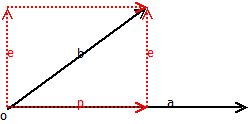
\includegraphics[width=0.8\textwidth]{images/gram-schmidt.png}
\end{center}
如图,将设两个不相关向量a、b,需要得到新的正交基$\hat{a}$、$\hat{b}$,从图中直观看到e与a正交,
求解e就是要的结果
\begin{gather*}
    \hat{e} = b - p = b - \frac{a^{T}b}{a^{T}a}a
\end{gather*}
当引入第三个不相关的向量c时,前面两个正交基求解不变,第三个分正交分量c为
\begin{gather*}
    \hat{c} = c - \frac{a^{T}c}{a^{T}a}a - \frac{b^{T}c}{b^{T}b}b
\end{gather*}
这样得到的向量就是最终的正交基,这个可以推广到N维向量。
\par
通过图示来解释一下求解的过程
\begin{center}
    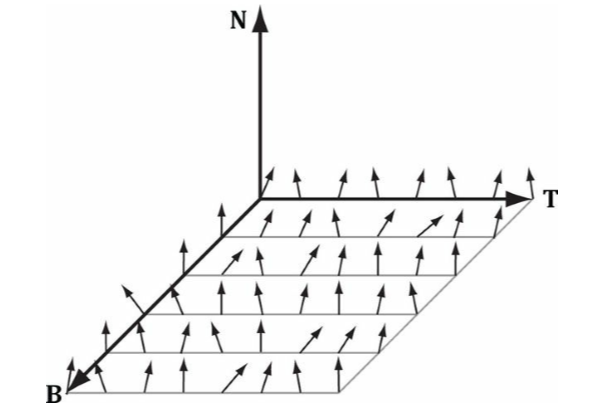
\includegraphics[width=0.8\textwidth]{images/normal_map_tnb.png}
    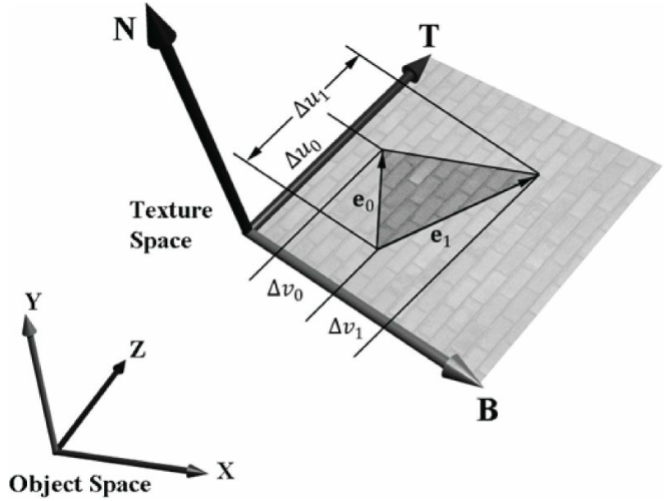
\includegraphics[width=0.8\textwidth]{images/normal_map_tnb_in_object_space.png}
\end{center}
假设三角形的三个顶点为$V_{0},V_{1},V_{2}$,对应的纹理坐标为$(u_{0},v_{0}),(u_{1},v_{1}),(u_{2},v_{2})$
\begin{gather*}
    \because \overrightarrow{e_{0}} = V_{1} - V_{0}, \overrightarrow{e_{1}} = V_{2} - V_{0} \\ 
    \therefore (\Delta u_{0},\Delta v_{0}) = (u_{1} - u_{0}, v_{1} - v{0}),
    (\Delta u_{1}, \Delta v_{1}) = (u_{2} - u_{0}, v_{2} - v_{0}) \\ 
    \therefore \overrightarrow{e_{0}} = \Delta u_{0} \ast \overrightarrow{T} + \Delta v_{0} \ast \overrightarrow{B}, 
    \overrightarrow{e_{1}} = \Delta u_{1} \ast \overrightarrow{T} + \Delta v_{1} \ast \overrightarrow{B} \\    
\end{gather*}
转换为向量表示他们的关系,再转换为矩阵形式,其中逆矩阵等于1除以原矩阵的行列式,再乘以它的伴随矩阵
\begin{gather*}
    \therefore \begin{bmatrix}
        \overrightarrow{e_{0}}.x & \overrightarrow{e_{0}}.y & \overrightarrow{e_{0}}.z \\ 
        \overrightarrow{e_{1}}.x & \overrightarrow{e_{1}}.y & \overrightarrow{e_{1}}.z  
    \end{bmatrix} = \begin{bmatrix}
        \Delta u_{0} & \Delta v_{0} \\ 
        \Delta u_{1} & \Delta v_{1}
    \end{bmatrix} \begin{bmatrix}
        \overrightarrow{T}.x & \overrightarrow{T}.y & \overrightarrow{T}.z \\ 
        \overrightarrow{B}.x & \overrightarrow{B}.y & \overrightarrow{B}.z  
    \end{bmatrix} \\ 
    \begin{bmatrix}
        \overrightarrow{T}.x & \overrightarrow{T}.y & \overrightarrow{T}.z \\ 
        \overrightarrow{B}.x & \overrightarrow{B}.y & \overrightarrow{B}.z  
    \end{bmatrix} = \begin{bmatrix}
        \Delta u_{0} & \Delta v_{0} \\ 
        \Delta u_{1} & \Delta v_{1}
    \end{bmatrix}^{-1} \begin{bmatrix}
        \overrightarrow{e_{0}}.x & \overrightarrow{e_{0}}.y & \overrightarrow{e_{0}}.z \\ 
        \overrightarrow{e_{1}}.x & \overrightarrow{e_{1}}.y & \overrightarrow{e_{1}}.z  
    \end{bmatrix} \\ 
    \because  \begin{bmatrix}
        \Delta u_{0} & \Delta v_{0} \\ 
        \Delta u_{1} & \Delta v_{1}
    \end{bmatrix}^{-1} = \frac{1}{\Delta u_{0} \Delta v_{1} - \Delta v_{0} \Delta u_{1}} \begin{bmatrix}
        \Delta v_{1} & -\Delta v_{0} \\ 
        -\Delta u_{1} & \Delta u_{0}
    \end{bmatrix} \\ 
    \therefore \begin{bmatrix}
        \overrightarrow{T}.x & \overrightarrow{T}.y & \overrightarrow{T}.z \\ 
        \overrightarrow{B}.x & \overrightarrow{B}.y & \overrightarrow{B}.z  
    \end{bmatrix} = \frac{1}{\Delta u_{0} \Delta v_{1} - \Delta v_{0} \Delta u_{1}} \begin{bmatrix}
        \Delta v_{1} & -\Delta v_{0} \\ 
        -\Delta u_{1} & \Delta u_{0}
    \end{bmatrix} \begin{bmatrix}
        \overrightarrow{e_{0}}.x & \overrightarrow{e_{0}}.y & \overrightarrow{e_{0}}.z \\ 
        \overrightarrow{e_{1}}.x & \overrightarrow{e_{1}}.y & \overrightarrow{e_{1}}.z  
    \end{bmatrix} 
\end{gather*}
根据以上公式就可以得到切线T和副法线B。这样就可以在vs中传入normal和tangent,并计算得到binormal,并把这三个向量
标准归一化后传给fs,构造TBN矩阵后乘以从bump map中拿到的法线相乘就是世界坐标的法线了,就可以直接参与光照计算了。
\par
简单地说一下光照中素级法线的用法,每个像素的颜色outColor = baseColor(ambient + diffuse ) + specular。用到像素法线的是
diffuse和specular,normal、view、halfViewAndLight三者的关系,就是夹角cos因子,要保证normal与view和halfViewAndLight是在
同一坐标系下且标准归一化的向量,夹角cos就是一定的。也就是把所有的计算都放在切线空间中,这需要把光线向量ray和视图向量view转换到
切线空间中,转换的公式是
\begin{gather*}
    \frac{view}{ray} \times TBN^{-1}
\end{gather*}
TBN矩阵的逆矩阵就是转置矩阵,因为构造TBN的都是标准归一化的正交矩阵,因为$\frac{view}{ray}$在vs中进行转换即可。

\par
这两种方法消耗都是2N次变换。追问一下像素切线与顶点切线空间的关系,下图是OpenGL中切线空间的位置:
\begin{center}
    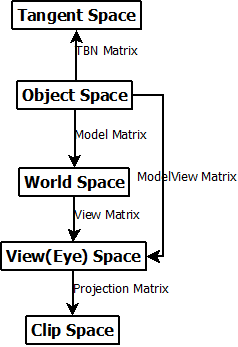
\includegraphics[width=0.8\textwidth,angle=270]{images/ShaderSpace.png}
\end{center}
TBN矩阵是从切线空间到模型空间的变换矩阵,其中的TBN
